%chapters/cs-uwb-pos.tex
\subsection{CS Receivers for UWB Positioning}
\begin{figure}[!t]
\centering
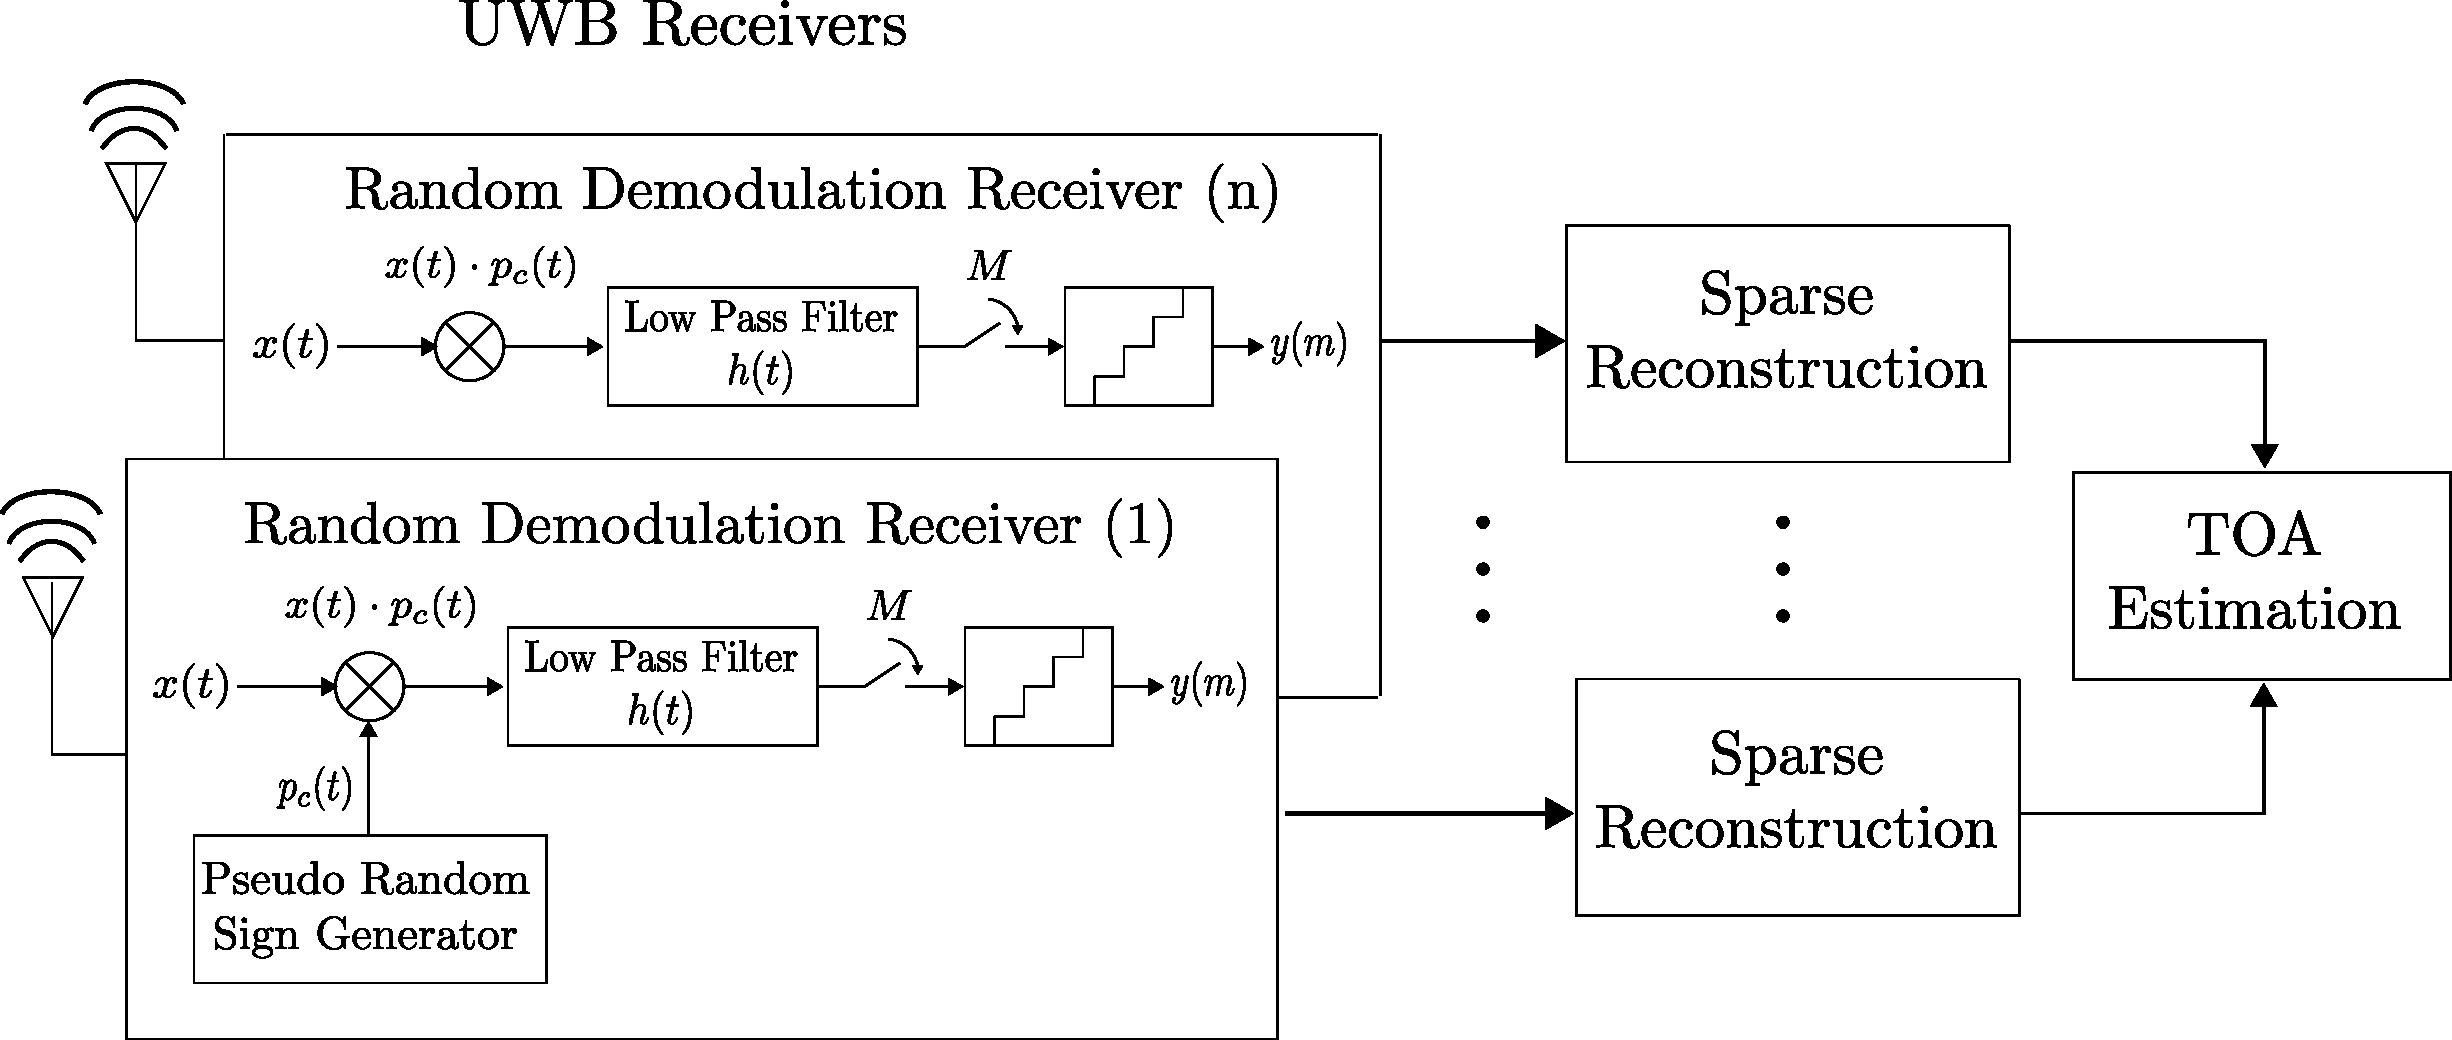
\includegraphics[width=3.5in]{cs-uwb-design1.pdf}
\DeclareGraphicsExtensions.
\caption{Block diagram of CS Receiver implemented by random demodulator (RD). The components of RD includes a pseudo-random sign generator (PRSG), a low-pass filter (LPF), and a sub-Nyquist ADC}
\label{cs-uwb-design1}
\end{figure}

Typical recent researches embed the CS reconstruction algorithm at UWB receivers to improve the SNR of the received signal. As a result, it not only increases the performance of the positioning accuracy \cite{banitalebi2014compressive}, but also reduces the sampling rate to a relatively low level compared to the Nyquist rate. Among these CS Receivers, most of them develop the random demodulator (RD) \cite{kirolos2006analog} as the main structure of CS based UWB receivers \cite{yang2011compressive}. 

In this system, each CS Receiver realizes the RD architecture that composed of a pseudo-random sign generator (PRSG), a low pass filter (LPF), and a sub-Nyquist rate analog-to-digital converter (ADC), shown in Fig.\ref{cs-uwb-design1}. 

Then the transmitted UWB signals are collected by group of low-rate distributed ADCs only using a minimal sampling rate of $1.7K(log(N/K))$ \cite{kirolos2006analog}, where $N$ stands for Nyquist rate and $K$ is the sparsity in transmitted UWB signals. Results in \cite{yang2013compressive} demonstrates that the new system successfully improves positioning accuracy. 

\subsection{CS Pre-Filtering for UWB Positioning}
On the other hand, some researches embed the CS technique at the UWB transmitter and regarded it as a better solution than CS receivers in terms of  system hardware power efficiency. The new architecture contains a random tap FIR at the transmitter, which acomplishes the CS random projection before UWB signals are transmitted \cite{zhang2009compressed}. Followed by distributed sub-Nyquist rate ADCs, the downsampled signals are collected for TOA based algorithm. Simulation result \cite{zhang2009compressed} shows that the new CS transmitter is suitable for detecting the indoor channel model with higher accuarcy than traditional TOA based method. This architecture is also suitable for indoor positioning because the transimitted signal pulse and channel model keep the same. Besides, it meanwhile saves more energy cost since it contains less hardware mixers than CS receiver based UWB system. However, the complexity of implementation a high data rate random tap FIR filters brings additional cost and becomes a main difficultiy in applications.

